\documentclass[tikz,convert={density=800,outext=.png},border=5pt]{standalone}
%\documentclass[preview,border=5pt]{standalone}

\usepackage[T2A]{fontenc}       			%поддержка кириллицы
\usepackage[utf8]{inputenc}					% Выбор языка и кодировки
\usepackage[english]{babel}

\usepackage{amsmath} % nice math symbols

\usepackage{tikz}
\usetikzlibrary{shapes,positioning,calc}

\begin{document}
	
	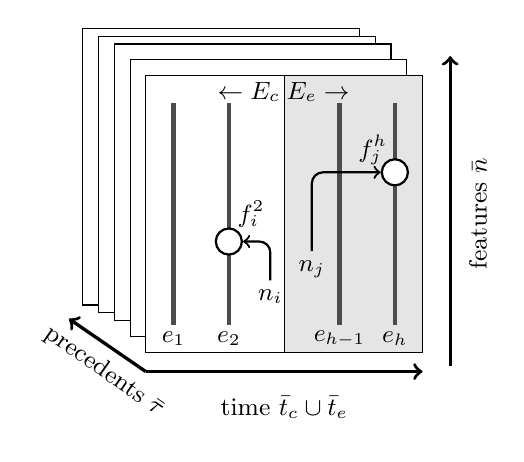
\begin{tikzpicture}
	\tikzstyle{z_pred}=[draw, rectangle,fill=white];
	
	\node[z_pred, minimum width = 100pt, minimum height = 100pt] (z_ex1) at ($(0,0)$) {};
	\node[z_pred, minimum width = 100pt, minimum height = 100pt] at ($(z_ex1)+(0.2,-0.1)$) {};
	\node[z_pred, minimum width = 100pt, minimum height = 100pt] at ($(z_ex1)+(0.4,-0.2)$) {};
	\node[z_pred, minimum width = 100pt, minimum height = 100pt] at ($(z_ex1)+(0.6,-0.4)$) {};
	\node[z_pred, minimum width = 100, minimum height = 100] (z_l_ex1) at ($(z_ex1)+(0.8,-0.6)$) {};
	\draw ($(z_l_ex1)+(0pt,50pt)$) -- ($(z_l_ex1)+(0pt,-50pt)$);
	\draw[draw, fill=white!90!black] ($(z_l_ex1)+(0pt,50pt)$) rectangle ($(z_l_ex1)+(50pt,-50pt)$);
	
	\draw[very thick, ->] ($(z_l_ex1)+(-50pt,-57pt)$) to ($(z_ex1)+(-55pt,-55pt)$);
	\draw[very thick, ->] ($(z_l_ex1)+(-50pt,-57pt)$) to ($(z_l_ex1)+(50pt,-57pt)$);
	\draw[very thick, ->] ($(z_l_ex1)+(60pt,-55pt)$) to ($(z_l_ex1)+(60pt,57pt)$);
	
	\node[align=center, font=\small] at ($(z_l_ex1)+(0,-70pt)$) {time $\bar t_c \cup \bar t_e$};
	\node[align=center, rotate=-35, font=\small] at ($(z_l_ex1)+(-65pt,-57pt)$) {precedents $\bar \tau$};
	\node[align=center, rotate=90, font=\small] at ($(z_l_ex1)+(70pt,0pt)$) {features $\bar n$};
	

	\draw[ultra thick, gray!60!black] ($(z_l_ex1)+(-40pt,40pt)$) -- ($(z_l_ex1)+(-40pt,-40pt)$);
	\draw[ultra thick, gray!60!black] ($(z_l_ex1)+(-20pt,40pt)$) -- ($(z_l_ex1)+(-20pt,-40pt)$);
	\draw[ultra thick, gray!60!black] ($(z_l_ex1)+(20pt,40pt)$) -- ($(z_l_ex1)+(20pt,-40pt)$);
	\draw[ultra thick, gray!60!black] ($(z_l_ex1)+(40pt,40pt)$) -- ($(z_l_ex1)+(40pt,-40pt)$);
	\node[align=center, font=\small] at ($(z_l_ex1)+(-40pt,-45pt)$) {$e_1$};
	\node[align=center, font=\small] at ($(z_l_ex1)+(-20pt,-45pt)$) {$e_2$};
	\node[align=center, font=\small] at ($(z_l_ex1)+(20pt,-45pt)$) {$e_{h-1}$};
	\node[align=center, font=\small] at ($(z_l_ex1)+(40pt,-45pt)$) {$e_h$};
	
	
	\node[align=center, font=\small] at (10pt,27pt) {$\leftarrow E_c$};
	\node[align=center, font=\small] at (35pt,27pt) {$E_e \rightarrow$};
	
	\node[align=center, font=\small] (s1) at ($(z_l_ex1)+(10pt,-20pt)$) {$n_j$};
	\node[align=center, font=\small] at ($(z_l_ex1)+(32pt,23pt)$) {$f_j^h$};
	\node[align=center, font=\small] (s2) at ($(z_l_ex1)+(-5pt,-30pt)$) {$n_i$};
	\node[align=center, font=\small] at ($(z_l_ex1)+(-12pt,0pt)$) {$f_i^2$};
	
	\node[draw, thick, align=center, fill=white, circle, minimum size=1pt] (p1) at ($(z_l_ex1)+(-20pt,-10pt)$) {};
	\node[draw, thick, align=center, fill=white, circle, minimum size=1pt] (p2) at ($(z_l_ex1)+(40pt,15pt)$) {};
	
	\draw[thick, <-,rounded corners] (p2.west) -| ($(z_l_ex1)+(10pt,0pt)$) |- (s1.north);
	\draw[thick, <-,rounded corners] (p1.east) -| ($(z_l_ex1)+(-5pt,-20pt)$) |- (s2.north);
		
	\end{tikzpicture}
	
	
\end{document}